\label{ch:introduction}
The SoA (service oriented architecture) design principle is a promising design philosophy, which features a lot of benefits and advantages over the static and vendor dependent architectures, which are implemented in today's vehicles. Hence, it is not surprising that there have already been various projects dealing with SoAs in real-time embedded systems. Those include SIRENA, SOCRATES, OASiS, MORE, RUNES and $\varepsilon$SOA \cite{scholz} \cite{sommer} \cite{buckl}. However, they do not address the necessary functional safety and fault tolerance requirements, which are preceding in vehicles. Work package 1, entitled ``Embedded System Architectures'', is dedicated to the investigation of these issues, because the SoA will give way to a new generation of vehicles, which are able to interconnect and operate autonomously.

One of the most important sources for this thesis was the \mbox{ISO 26262} standard. Emerging from the \mbox{IEC 61508} standard, the \emph{ISO 26262} standard is an international functional safety standard for series production passenger cars with a maximum gross weight of 3.500kg. It is the state of the art for vehicles and does not set any requirements in terms of performance of equipment, but is only concerned with possible malfunctions. In total the standard features ten parts. Of enhanced relevance have been \textbf{part 1}, which defines all the related terms and vocabulary, \textbf{part 3} which deals with the \textbf{concept phase}, and \textbf{part 4}, which is dedicated  to the development at system level \cite{iso26262:1} \cite{iso26262:3} \cite{iso26262:4}.

The standard does not issue any regulations concerning SoA, but only provides certain requirements, which have to be fulfilled. However, there are no prescriptions on how they should be achieved \cite{iso26262:course1}.

Another important source of information was AUTOSAR. The term AUTOSAR is ambiguous, for it can denote either the technical product (\textbf{AUT}omotive \textbf{O}pen \textbf{S}ystem \textbf{AR}chitecture), or the related development partnership \cite{autosar_rs_main}. The partnership was founded in 2003, with its members covering more than 80\% of the production of cars worldwide \cite{kirschke_biller2011} \cite{schmerler2012}. They provide a standard, which aims at establishing an industry norm for automotive software architecture. This allows different partners, as well as suppliers and manufacturers, to collaborate without any obstacles in terms of languages or methodologies. In detail, this is achieved by the definition of a unified \emph{software architecture} and \emph{software development methodology}, as well as \emph{standardised application interfaces}. By stressing the decoupling of hardware and software the standard gives way to software reuse on different hardware platforms \cite{kirschke_biller2011} \cite{schmerler2012}, what is in compliance with the SoA design principles. Thus, many of the terms, treated within this thesis are influenced by AUTOSAR.

The remain of chapter \ref{ch:introduction} contains a definition of the most important terms related to SoA. Those terms include \emph{system}, \emph{component}, \emph{service}, \emph{architecture}, \emph{service oriented architecture}, \emph{dependability} and \emph{functional safety}. Each of the following sections starts with an investigation and comparison of definitions from different sources. Subsequently, a definition, which is in accordance with the context of safety-critical embedded systems is presented in a bordered box. Finally, some additional information related to the particular term may follow.






\section{System}
\label{ch:system}
Obermaisser and Kopetz describe in their GENESYS reference architecture a system as ``an entity that is capable of interacting with its environment and is sensitive to the progression of time'' \cite[p.7]{genesys}. The environment is thereby a system itself, which produces input for other systems and acts according to their outputs. Which elements (cf. section \ref{sec:system_element}) belong to the system, and which to the environment, is a matter of perspective. 

In the \mbox{ISO 26262} standard, a system is referred to as a ``set of elements that relates at least a sensor, a controller and an actuator with one another'' \cite{iso26262:1}. This definition is obviously referring explicitly to automotive, because in other industry sectors a system does not necessarily contain actuators.

According to AUTOSAR, a system is ``an integrated composite that consists of one or more of the processes, hardware, software, facilities and people, that provides a capability to satisfy a stated need or objective'' \cite{autosar_glossary}.

Other typical characteristics are the presence of some kind of internal structure and the hierarchical composition. Those are included in the resulting definition below.

\begin{myquote}
A system is a hierarchical composed, time sensitive element, which interacts with the environment by processing input and providing output in turn.

It is concerned with satisfying a specific need or purpose and disposes of a, more or less complex, internal structure, which may include hardware, software and data.
\end{myquote}

For the scope of this thesis, the overall system is assumed to be a vehicle, if not stated otherwise. The environment consists therefore of other vehicles and the surrounding infrastructure. Nevertheless, the entire traffic could also be taken as a system and the environment would then be a different one.



\subsection{System Element}
\label{sec:system_element}
In the \mbox{ISO 26262} standard system elements are described as ``system or part of system including components hardware, software, hardware parts, and software units'' \cite{iso26262:1}. It is a very generic term and does not refer to any entities at a specific layer or with a specific characteristic. Instead, it can be more or less any entity of a system, since a system itself is defined as set of elements \cite{iso26262:1}. Figure \ref{fig:26262_disambiguation} pictures the relations to other terms and should serve as naming convention throughout this thesis.

\begin{figure}[!htbp]
\centering
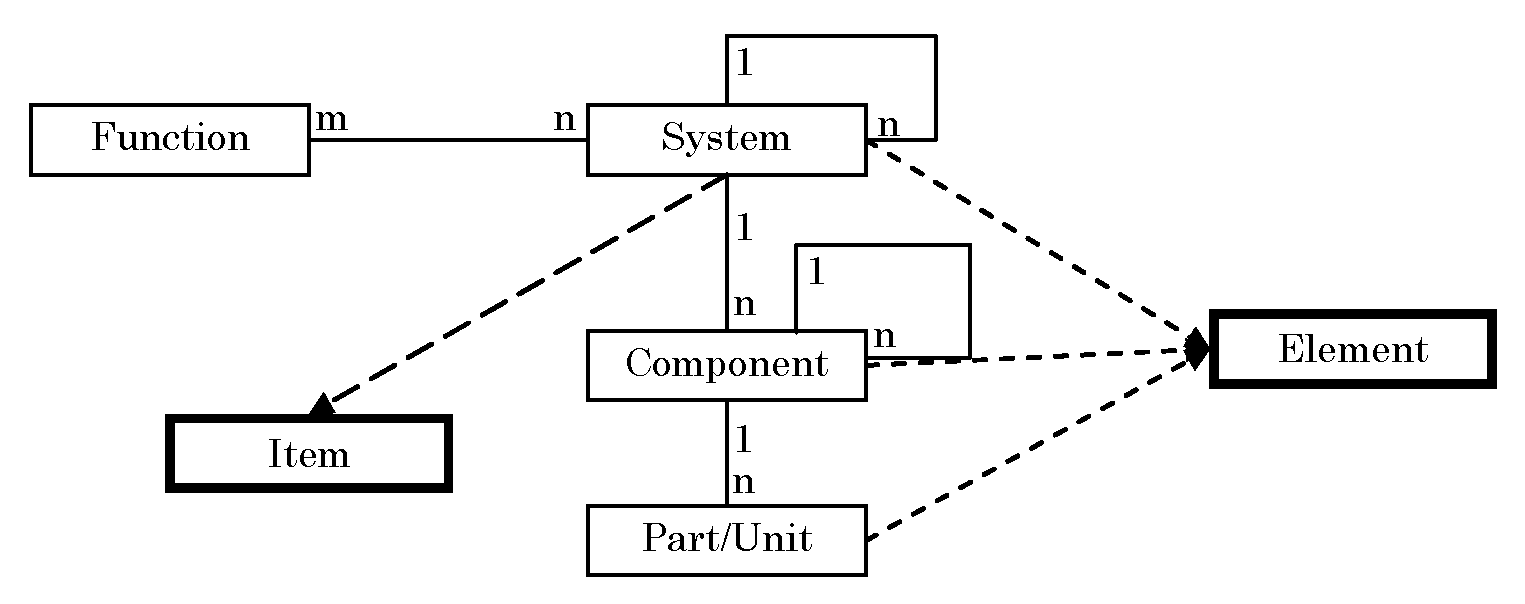
\includegraphics[scale=0.5]{26262_disambiguation_system_etc.pdf}

\caption{Relation of \emph{system}, \emph{component} and \emph{element} according to ISO 26262 \cite{iso26262:course1}.}
\label{fig:26262_disambiguation}
\end{figure}


\subsection{System of Systems}
Systems are hierarchical and can be composed or decomposed into sets of interacting constituting systems. Often this is referred to by the term \emph{System of Systems (SoS)} \cite[p.7]{genesys}. Thus, the SoS is in general the level above a given system and is therefore dependent on the definition of the related systems. SoSs may be geographically distributed and can become parts of other, bigger SoSs, when collaborating with other SoSs.

For a system vehicle, a SoS could be for example the traffic of a city, with many vehicles participating.


\subsection{System Layers}
\label{ch:system_layers}
The parts of a system can be divided into different layers of implementation. This kind of abstraction enables the comprehension of the overall relations. Unfortunately each field of research features its own, sometimes even contradicting, way of fractionising systems.
\\
\\
The GENESYS architecture by Obermaisser and Kopetz distinguishes between three different layers, denoted \emph{chip-level}, \emph{device-level} and \emph{system-level} \cite[p.44]{genesys}. An example of the hardware elements at different levels by means of a system vehicle can be seen in figure \ref{fig:integration_levels}.
\begin{description}
\item [System Level.]
The system level consists of \emph{Devices}, which are themselves logically self-contained apparatus. With respect to a system vehicle this could be for example an ECU, a sensor, an actuator or the like \cite[p.45]{genesys}.
\item [Device Level.]
The devices at the system level, contain a certain internal structures themselves. In case of embedded systems these are in most cases \emph{Chips} \cite[p.45]{genesys}, like the the AURIX\textsuperscript{TM} chip, which is frequently used in the automotive industry.
\item [Chip Level.]
According to the implementation layers in the GENESYS architecture, the chip level is the lowest level of implementation. In case of an MPSoC (Multiprocessor System-on-Chip) this level contains the single IP Cores of the chip \cite[p.46]{genesys}
\end{description}

\begin{figure}[!htbp]
\centering
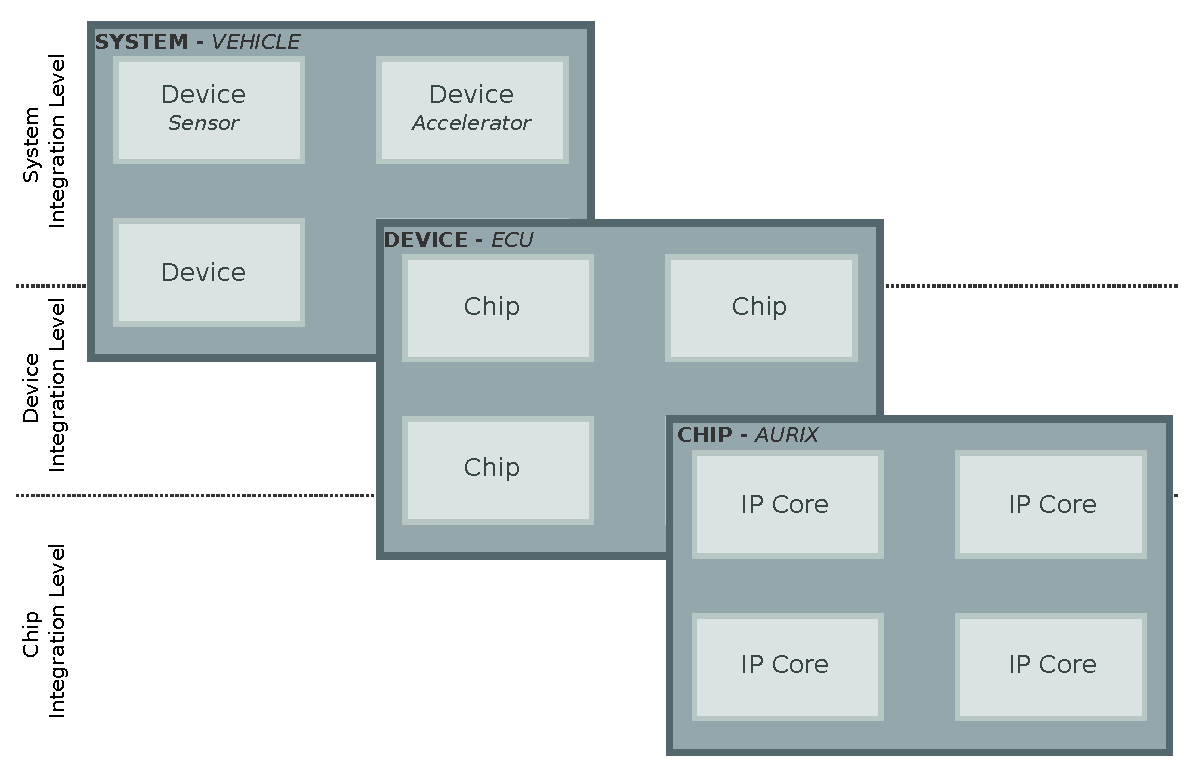
\includegraphics[width=\textwidth]{system_levels.pdf}
\caption{The hierarchy of the implementation layers of the system vehicle with examples.}
\label{fig:integration_levels}
\end{figure}

The Arrowhead Framework provides an hierarchy by means of documentation documents, which are spitted in the three levels \emph{system-of-systems}, \emph{system} and \emph{service} \cite{arrowhead_inpr}. Their involved documents and relations are pictured in figure \ref{fig:sys-arrowhead}.

\begin{description}
\item [System-of-systems.] The levels features the two documents \emph{SoS Description (SoSD)} and \emph{SoS Design Description (SoSDD)}. They differ in the amount of information they are revealing. While the first represents only an abstract view, the second also reveals the implementation of the SoS and its technologies \cite{arrowhead_inpr}.
\item [System.] The system level comes with the two documents \emph{System Description (SysD)} and \emph{System Design Description (SysDD)}. Just as at the SoS level the first one features a kind of black box opacity and the second a white box view \cite{arrowhead_inpr}.
\item [Service.] The service level contains the four documents \emph{Service Description (SD)}, \emph{Interface Design Description (IDD)}, \emph{Communication Profile (CP)} and \emph{Semantic Profile (SP)}. The service description is referred to in \ref{sec:service_structure}.
\end{description}

\begin{figure}[!htbp]
\centering
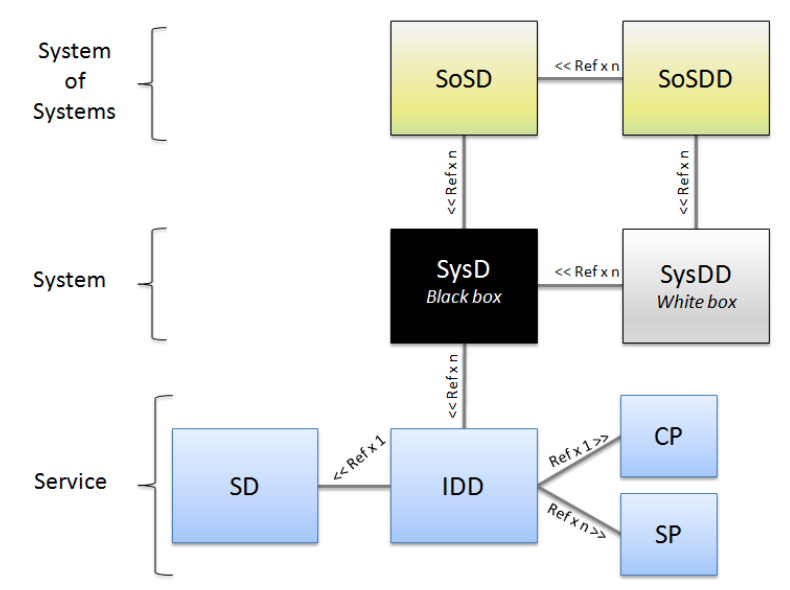
\includegraphics[scale=0.4]{arrowhead-documentation-relationship.png}
\caption{Relation of System, SoS and Service to one another \cite{arrowhead:presentation}.}
\label{fig:sys-arrowhead}
\end{figure}

All the documents exist as templates which should be filled out during the development process of a system. They feature a XML like style in order to be human and machine readable at the same time.

Developed systems can then be constituted to SoS by an underlying cloud, as depicted in figure \ref{fig:arrowhead-framework}. All the system have specified and standardised interfaces and work together by means of three \emph{core services}, labeled II, AI and SM.
\begin{description}
\item [Information Assurance (IA).]
This service is responsible for providing secure information exchange through authorization and authentication \cite{arrowhead:presentation}.
\item [Information Infrastructure (II).]
The II service enables the listing of the services in the \emph{service repository} (cf. section \ref{sec:structure_of_soa}) and their discoverability \cite{arrowhead:presentation}.
\item [System Management (SM).]
This is the core service for the system of systems composition and features logging and monitoring abilities \cite{arrowhead:presentation}.
\end{description}

\begin{figure}[!htbp]
\centering
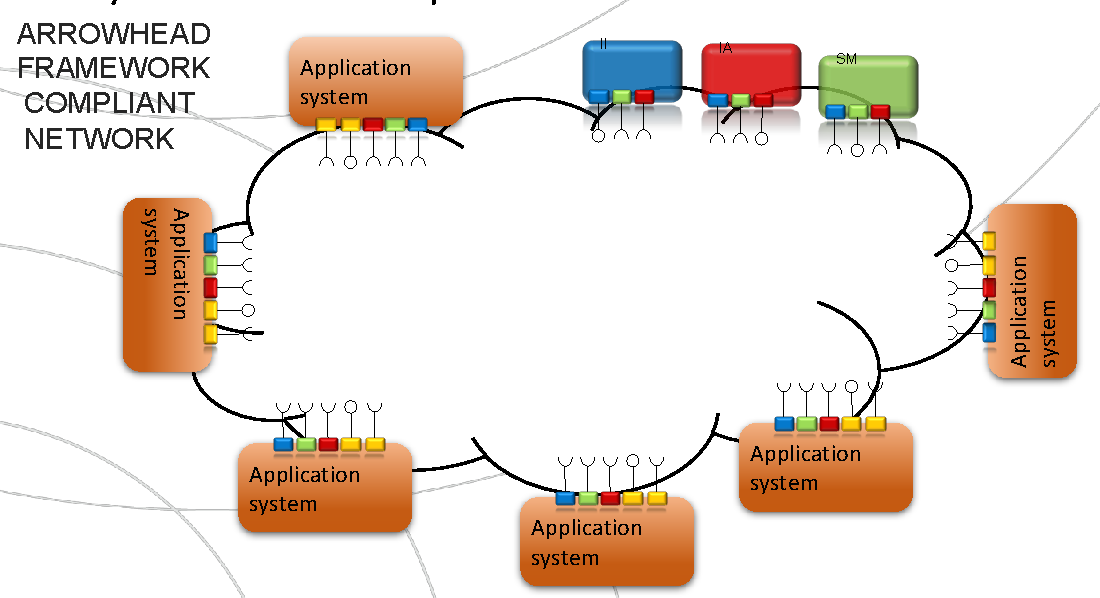
\includegraphics[scale=0.8]{arrowhead-framework.pdf}
\caption{Implementation example of an ARROWHEAD framework \cite{arrowhead:presentation}.}
\label{fig:arrowhead-framework}
\end{figure}

When comparing these two approaches by GENESYS and ARROWHEAD, it becomes obvious that the latter has a quite abstract point of view, which is bias towards SoA, while the approach by GENESYS is much more hardware oriented.



\subsection{Embedded System}
\label{sec:embedded_system}

Embedded systems (ES) are computational modules integrated to physical devices and equipment. The have a predefined set of tasks and requirements and are capable of processing information \cite{rodrigues2011} \cite[p.xiii]{marwedel}. Compared to general-purpose computation systems they usually dispose of less processing resources and come with narrower operation ranges, but at the same time they feature a high efficiency by optimally managing the available resources \cite[p.283]{alippi} \cite[p.5]{marwedel}. Also, their presence is usually quite unobtrusive, because instead of mouse and keyboard the user interface consists of typical input devices like buttons, steering wheel, or pedals.

ESs are reactive systems, what means that they perform a continuous interaction with the environment. The connection to the physical environment is realised by means of sensors, responsible for collecting information, and actuators for performing the actual reaction \cite[p.8-9]{marwedel}. 

During operation, they are in a certain state and waiting for input. When provided with that, they perform computations and generate an output, which is handed back to the environment \cite[p.9]{marwedel}. ESs in safety-critical applications have to care about the issues \emph{time constraints}, \emph{dependability} and \emph{efficiency requirements}.

\begin{description}
	\item [Time constraints.]
	One challenge of Embedded Systems is the meeting of so called \emph{time constraints}, which basically means the conduction of a computation within a specified time \cite[p.8-9]{marwedel} \cite{rodrigues2011}. Kopetz states ``A time-constraint is called hard if not meeting that constraint could result in a catastrophe'' \cite{kopetz}.
	\item [Dependability.]
	Embedded systems, operating in safety-critical environment, like nuclear power plants, cars, trains or aircraft, must be \emph{dependable}, for they are directly connected to the environment and have immediate impact on it. The Dependability is split up in further aspects. In detail, those are \emph{Reliability} (cf. section \ref{sec:reliability}), \emph{Maintainability}, \emph{Availability} (cf. section \ref{sec:availability}), \emph{Safety} (cf. chapter \ref{ch:functional_safety}) and \emph{Security} \cite[p.4-5]{marwedel}.
	\item [Efficiency requirements.]
	Efficiency is a key concept of embedded systems and is concerned with providing a maximum computation performance while minimizing the required energy. The efficiency is measured in ``operations per Joule'' and has been been increasing almost exponentially during the last twenty years \cite{marwedel}.
\end{description}






\section{Component}
\label{ch:component}

The term component often appears in connection with SoA and frequently leads to confusion when it is put on a level with service (cf. chapter \ref{ch:service}). This ambiguity is a result of the historic development of the service oriented architecture as successor of the component based software engineering (CBSE).

Obermaisser and Kopetz state that a component is a software or hardware unit that performs a specified computation within a given period of time \cite[p.38]{genesys} and communicates with other components by means of specific \emph{interfaces} (cf. section \ref{sec:component_interfaces}). Like systems, components are hierarchical and therefore dependent on the point of view - from a different viewpoint a quantity of components may be seen as a single component. The ISO 26262 standard is in accordance with this definition and describes components as ``non-system level element that is logically and technically separable and is comprised of more than one hardware part or one or more software units'' \cite{iso26262:1}.
AUTOSAR, in contrast, refers to component explicitly as a part of software:	
\begin{quote}
``Software-Components are architectural elements that provide and/or require interfaces and are connected to each other through the Virtual Function Bus to fulfill architectural responsibilities'' \cite{autosar_glossary}.
\end{quote}
Hence, a software component is an encapsulation for parts of the automotive functionality, but there is no specific granularity dictated, meaning that an AUTOSAR software component might be either a ``small, reusable piece of functionality (such as a filter) or a larger block encapsulating an entire subsystem'' \cite{autosar}.

\begin{myquote}
A component is a logical and technical separable hardware or software unit that is capable of performing a specific computation.

It offers an abstraction that simplifies the understanding of complex systems. Therefore they have to be hierarchical, meaning that components can be composed to other, larger, components.
\end{myquote}

As suggested by this definition the term component may be used for both, software hardware. 
A component can be seen as black box, meaning that the more or less complex internal structure is invisible or not of concern for the user. Thus, other components stay unaffected from modifications of this internal structure, given that the behaviour at the \emph{Linking Interface} (cf. section \ref{sec:component_interfaces}) remains unchanged \cite[p.38-39]{genesys} \cite{autosar_intro} \cite{sametinger}. As a self-contained subsystem, it can be developed and tested independently, and latter be used as building block for systems or higher level components. In other words, the components are the basic building blocks of a system \cite{ning}. 

Nevertheless, not everything is a component. According to Sametinger, an algorithm in a book is not a component, but it has to be implemented by means of an arbitrary programming language and equipped with well-defined interfaces in order to become a component \cite[p.2-3]{sametinger}.


\subsection{Component Interfaces}
\label{sec:component_interfaces}
The interfaces are necessary for any interaction with other components.

Following the definition from Obermaisser and Kopetz, each component may dispose of up to four interfaces for communication with other entities. The \emph{Linking Interface}, the \emph{Local Interfaces} and the \emph{Technology Independent-} or \emph{Technology Dependent Interface}. They are illustrated in figure \ref{fig:component_interfaces} \cite[p.40-41]{genesys}.

\begin{description}
\item [Linking Interface (LIF).] 
The \emph{Linking Interface} is a message based interface and responsible for offering the component's services. The LIF is dependent on the level of integration, e.g. Inter-IP Core LIF at chip level or Inter-Chip LIF at device level. Nevertheless, it is used only for communication to other components at the same layer and also the only place, where a component may provide its services to other components \cite[p.9]{genesys}.

The \emph{Linking Interfaces} are always technology agnostic, which means that they do not expose details on their implementation or \emph{Local Interfaces}. Accordingly, the implementation can be modified, without other components noticing, as long as the specification at the LIF remains unchanged \cite[p.9, 40-41]{genesys}.

\item [Local Interface.] 
The \emph{Local Interfaces} establish the connection between a component and its local environment, which could consist of sensors, actuators and the like. If the environment is modified, the semantics and timing of the data should stay the same in order to do not violate the specification. A \emph{Local Interface} could also be mapped to a \emph{LIF} of a component at the next-higher level - this is known \emph{gateway component} and enables different layers to communicate with each other.

Components do not necessarily require local interfaces. Such are denoted \emph{Closed Components} \cite[p.40-41]{genesys}.

\item [Technology Independent Interface (TII).]
The \emph{TII} is the instrument for configuring and reconfiguring a component, e.g. assigning a name, configuring input and output ports or monitoring the resource management. Starting, restarting and resetting the component is also executed through this interface. The TII communicates with the hardware, the operating system and the middleware, but not with the \emph{application software (service)}, which is reserved for the LIF \cite[p.40-41]{genesys}.

\item [Technology Dependent Interface (TDI).] 
The \emph{Technology Dependent Interface} enables a look inside the component and allows to inspect internal variables and processes. Thus, it is reserved for people who bring a deep understanding of the components internals and is of no relevance for the user of the LIF services \cite[p.40-41]{genesys}. 
\end{description}

\begin{figure}[!htbp]
\centering
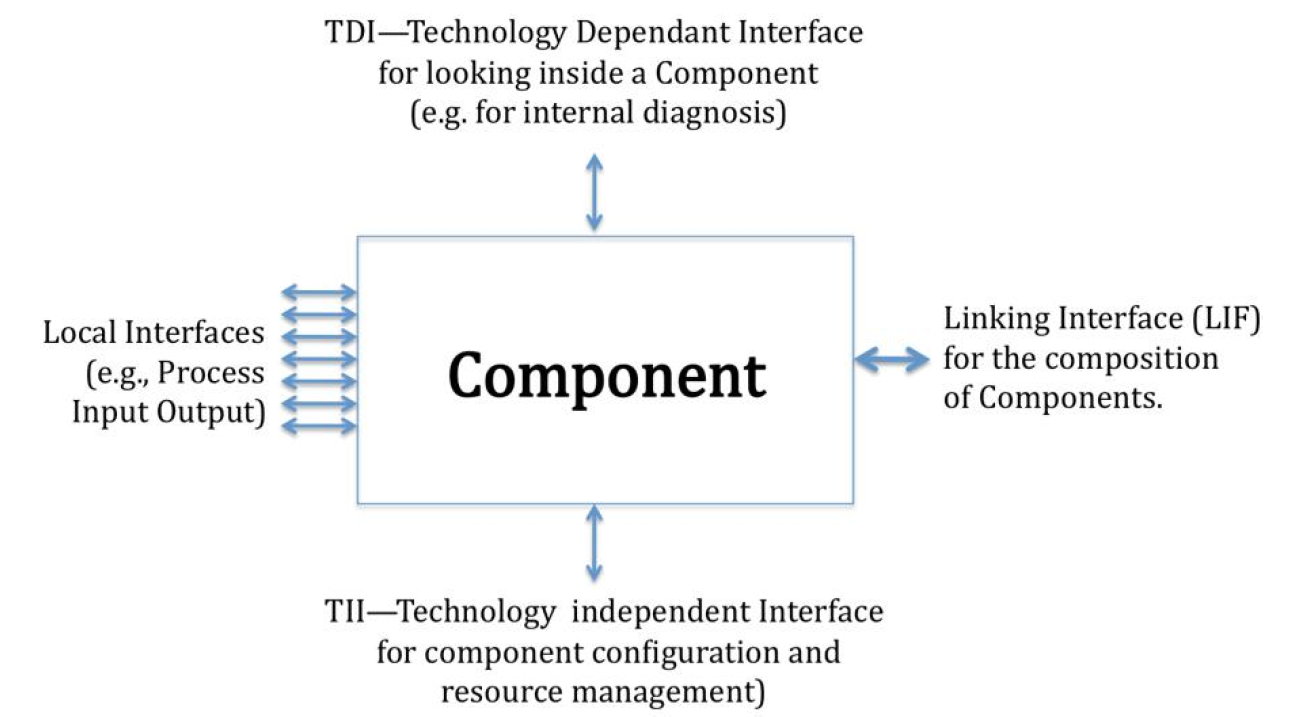
\includegraphics[scale=0.4]{component_interfaces.png}
\caption{The interfaces of a component, with respect to the GENESYS architecture \cite[p.40]{genesys}}
\label{fig:component_interfaces}
\end{figure}

Compared to this rather implementation oriented definition by GENESYS, the approach by AUTOSAR is much more abstract. According to their definition, a component may dispose of a number of ports. A port belongs to one component only and is the interface a component uses to communicate with other components. Within this context, the term interface specifies a kind of contract or specification, on which services can be called at this port, and the format of the data emitted at this port. There are four different types of interfaces, belonging to the two different communication patterns \textbf{Client-Server} and \textbf{Sender-Receiver} \cite{autosar_intro}:

\begin{description}
\item [Client-Server Communication.]
When this kind of communication is performed the \emph{client-component} requests a specific service from the \emph{server-component} and sends necessary parameters. The server then processes the incoming request and returns a response. A single component can be a server and a client at the same time \cite{autosar_intro}. A schematic illustration of this type of communication is pictured in figure \ref{fig:autosar_client-server}, where SW-C denotes \emph{software component}.

\item [Sender-Receiver Communication.]
The \emph{Sender-Receiver} approach is a bit different. The task of the sender is to distribute his information to one or more receivers, without ever getting a response in form of data or control flow. In fact he does not even know the number or identity of the receivers. Those have to decide on themselves, how to deal with the received data (cf. figure \ref{fig:autosar_sender-receiver}) \cite{autosar_intro}.
\end{description}

\begin{figure}[!htbp]
\centering
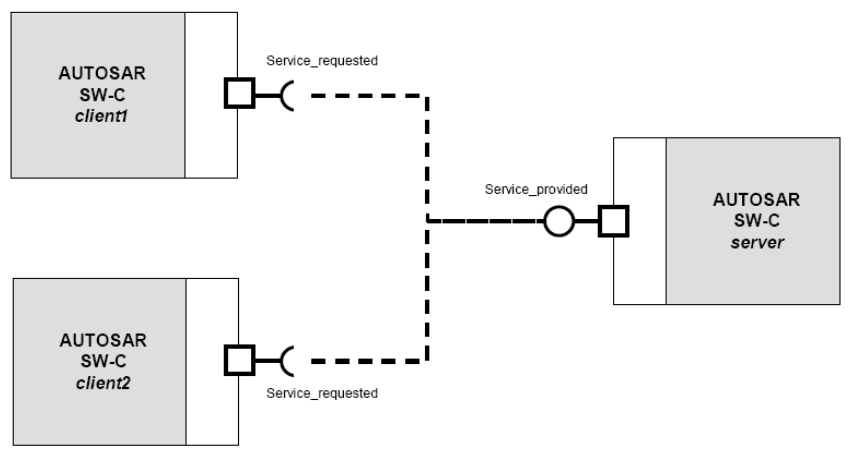
\includegraphics[scale=0.4]{autosar_client-server.png}
\caption{Illustration of the client-server communication \cite{autosar_intro}.}
\label{fig:autosar_client-server}
\end{figure}

\begin{figure}[!htbp]
\centering
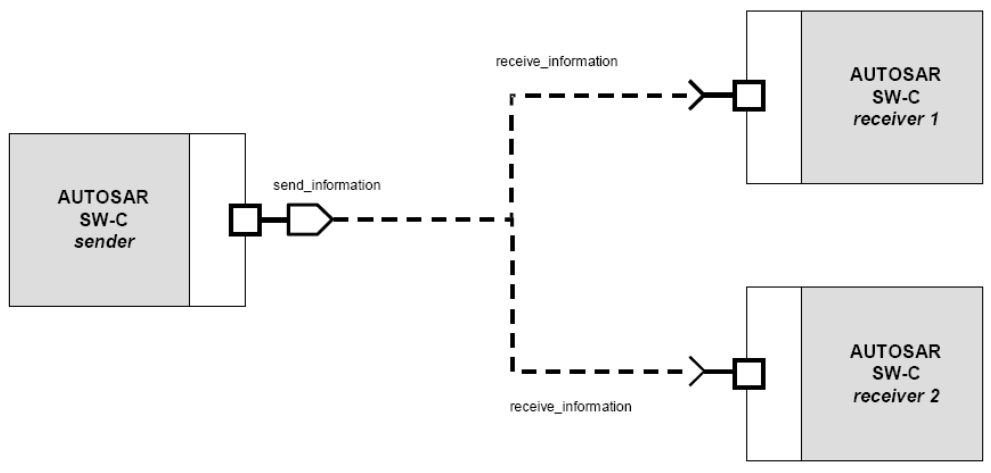
\includegraphics[scale=0.4]{autosar_sender-receiver.png}
\caption{Illustration of the sender-receiver communication \cite{autosar_intro}.}
\label{fig:autosar_sender-receiver}
\end{figure}










\section{Service}
\label{ch:service} 
The perception of the term \emph{service} is quite wide spread and influenced by a persons experience and environment (e.g. related research area, etc.). Unsurprisingly, numerous different perceptions emerged, supporting various even contradicting views.

The perhaps most generic definition of service is given by Arcitura \cite{arcitura}:
\begin{quote}
``Each service is assigned its own distinct context and is comprised of a set of capabilities related to this context. Therefore, a service can be considered a container of capabilities associated with a common purpose (or functional context).''
\end{quote}
The key information in this quote is that a service may offer multiple capabilities.

By Arrowhead a service is referred to as a part of a SoA \cite{arrowhead}:
\begin{quote}
``A service is the core building block of SOA, and is basically a software application performing some task, with a formal interface described using a standard description framework.''
\end{quote}

The definition by Obermaisser and Kopetz describes a service by means of its surrounding environment \cite[p.8]{genesys}:
\begin{quote}
``A service is what a system delivers to its environment according to the specification. Through its service, a system can support the environment, i.e., other systems that use the service.''
\end{quote}
What the specification of a service may look like is referred to in \ref{sec:service_structure}. While it is indicated that a service interacts somehow with its environment. By bringing in the concept of interfaces, AUTOSAR gives an answer to the question how and where this interaction is conducted \cite{autosar_glossary}:
\begin{quote}
``A service is a type of operation that has a published specification of interface and behaviour, involving a contract between the provider of the capability and the potential clients.'' 
\end{quote}
The terms \emph{contract}, \emph{provider} and \emph{client}, which also appear in the definition below are investigated in detail in section \ref{sec:structure_of_soa}.

\begin{myquote}
	As part of a system, a service is an independent logical unit with at least one capability and well defined interfaces, which have to be fully described by the service contract.

	Services are the building blocks of a service oriented architecture and the containers for the functionalities a service provider offers to its consumers.

	In order to be applied in a service oriented architecture, a service must comply with certain key concepts.
\end{myquote}



\subsection{Key concepts of a service}
\label{sec:service-concepts}
Erl, Bennett et al. \cite[p.27]{erl2011} state eight specific characteristics any service should posses. Those have been altered and extended with some attributes from other sources, resulting in the following listing with a total of nine characteristics. In some occasions there have been different nominations of equal characteristics. In those cases all alternative naming are stated as well.

\begin{description}
\item [Opacity/ Encapsulation/ Abstraction.]
According to Erl, abstraction means to ``hide information about a program not absolutely required for others to effectively use that program'' \cite[ch.8.1.]{erl2008}.
Services hide an internal logic, which could be implemented by means of any suitable programming language or operating system. This allows the logic and implementation of the service to evolve over time, while still providing the functionality as it was originally published \cite[ch.8.1]{erl2008}.

From the service consumer's point of view the service appears as a black box, which does not impart anything of the underlying implementation or how the returned information is generated \cite{opengroup} \cite{breivold} \cite{arrowhead} \cite[p.27]{erl2011}.

This black box encapsulation disables any modification of the service by the user and is often referred to as \emph{service interface level abstraction} \cite{breivold}.

\item [Reusability.]
The idea of software reuse is present since the early days of software engineering. In SoAs it is the key concept of a service and a necessary basis, for many of the other concepts would not even be possible without it \cite[ch.9.1.]{erl2008} \cite[p.27]{erl2011}.

This design principle aims at making a service applicable for more than just one specific use case. Usually, it results in a more generic programming logic, which allows a wider range of application.

It should be noted, that the terms reusability and reuse are not equal. The former is the design principle, while the latter denotes the result which should be achieved by applying the concept of reusability.

\item [Composability.] 
Service are building blocks and thus existing services can be used in order to compose other, possibly more advanced, services through service orchestration or service choreography. 

With orchestration, one service acts as a coordinator between all services involved, in contrast to choreography, where all composed services work independently with each other in a completely distributed manner \cite{opengroup} \cite{arrowhead} \cite{breivold} \cite[p.27]{erl2011}.

In SoAs the composing may take place at runtime \cite{breivold}.

\item [Loose coupling.]
If two or more artefacts are somehow connected within a technical context, this is referred to by the term coupling. It indicates that two or more of ``something'' exist and is a measurement of the strength of their relationship, which is given by the amount of dependencies \cite{erl2008}.

SoAs should feature a loose coupling, which means that dependencies should be reduced as far as possible \cite{erl2008}. This is achieved by using standardised interfaces, what offers the service providers great flexibility in choosing design and deployment environment for offering their services \cite{breivold} \cite{arrowhead}. Well defined interfaces also allows a simple exchange of components by components from different vendors \cite{scholz}.

An example for this concept are web browsers. The service a web browser provides to the end user could be described as ``interpret the HTML files and illustrate them in a user friendly way''. No matter which web browser is used, the end result will stay almost unaffected thanks to the well specified applied protocols.

\item [Discoverability.] 
The concept of discoverability comes with certain requirements:
	\begin{itemize}
	\item services have to constantly communicate the meta information they want to make public and all alternations,
	\item this information should be centrally stored and maintained in consistent format and
	\item the meta information must be accessible and searchable by those who want to use this resource \cite[ch.12.]{erl2008}.
	\end{itemize}
The artefact that stores the service information in SoAs is the \emph{service repository} (cf. section \ref{sec:structure_of_soa}).

The discoverability of a service is not only critical during the runtime of a SoA, but also during the development process, where it provides answer to the question whether a certain functionality already exists or has to be built. Thereby redundancies are reduced or prevented altogether \cite[ch.12]{erl2008} \cite{arrowhead} \cite{breivold} \cite[p.27]{erl2011}.

\item [Self-description.]
Service provider have to provide their clients with all the relevant information in form of a service description. This includes syntax, semantic and behaviour \cite{breivold}.

\item [Statelessness.]
A state is referred to as the general condition of something. In computational systems a state can be represented by temporary data describing the state. SoA services are frequently required to hold a certain amount of state information through the lifespan of a service composition in order to fulfil their functionality \cite[ch.11]{erl2008}. 

Nevertheless, services can also be stateless and in order to optimise reusability services should aim at minimizing their state information and their holding time for messages \cite{breivold} \cite[p.27]{erl2011}.

\item [Technology neutrality.]
Services should be independent from used technology in order to allow different platforms to use them \cite{breivold}. 

This concept is questionable in connection with automotive, because in a car most of the implemented technology is given by certain standards and cannot be changed easily.

\item [Standardised Service Contract.]
According to Erl, ``Services within the same service inventory are in compliance with the same contract design standards'' \cite[p.27]{erl2011}. In other words, the service contract should be created by means of a given templates. The term \emph{service inventory} is referred to in \ref{sec:structure_of_soa}.
\end{description}



\subsection{Structure of a Service}
\label{sec:service_structure}
Concerning the structure, Krafzig describes a service as it can be seen in figure \ref{fig:service} with the artefacts \emph{service contract}, \emph{interface}, \emph{implementation}, \emph{business logic} and \emph{data} \cite[p.44]{krafzig}.

\begin{description}
\item [Service contract.] 
\begin{quote}
\emph{``A contract for a service (or a service contract) establishes the terms of engagement, providing technical constraints and requirements as well as any semantic information the service owner wishes to make public''} 
\cite[ch.6.1]{erl2008}.
\end{quote}
The service contract is, more or less, the core part of every service, for it is the complete specification of the service between a provider and a consumer. It provides all the meta information concerning functionality, capabilities, expected behaviour, constraints, service owner, access rights, functional and non functional qualities and information about intended performance and scalability of the service \cite[p.44]{krafzig} \cite[p.26]{josuttis} \cite{breivold}.

Physically, it is represented by one or more \emph{service description documents}, which should be human- and machine readable at the same time. This is the reason, why web services are usually represented by WSDL documents \cite[p.43]{erl2011}. There is no dedicated language standard for automotive yet, but a XML based language would be an appropriate choice.

Erl \cite{erl2008} distinguishes between technical and non-technical service description documents. If a \emph{consumer} connects to a \emph{provider}, for example a database, the technical contract could contain information like the database protocol and the query syntax or language, while the non-technical contract could contain related meta information like required safety measures or the physical location of the database \cite[ch.6.1]{erl2008}.

\item [Interface.] 
The interface is described in the service contract and specifies the access points and the functionality of the service to the customers, which are connected via a network. A service may dispose of multiple interfaces \cite[p.44]{krafzig} \cite{breivold}.

\item [Implementation.] 
The implementation is realised by programmes, configuration data and databases, which are necessary to provide the functionality specified in the contract. The term business logic in figure \ref{fig:service} is a bit misleading. This should be seen as the algorithms encapsulated in the implementation \cite[p.44]{krafzig}.

\item [Data.]
As stated in \ref{sec:service-concepts}, a service may dispose of some state data for the time of its application. However, this is no necessary requirement for a service and the amount of stored data should be kept as low as possible \cite[p.44]{krafzig}.
\end{description}

\begin{figure}[!htbp]
\centering
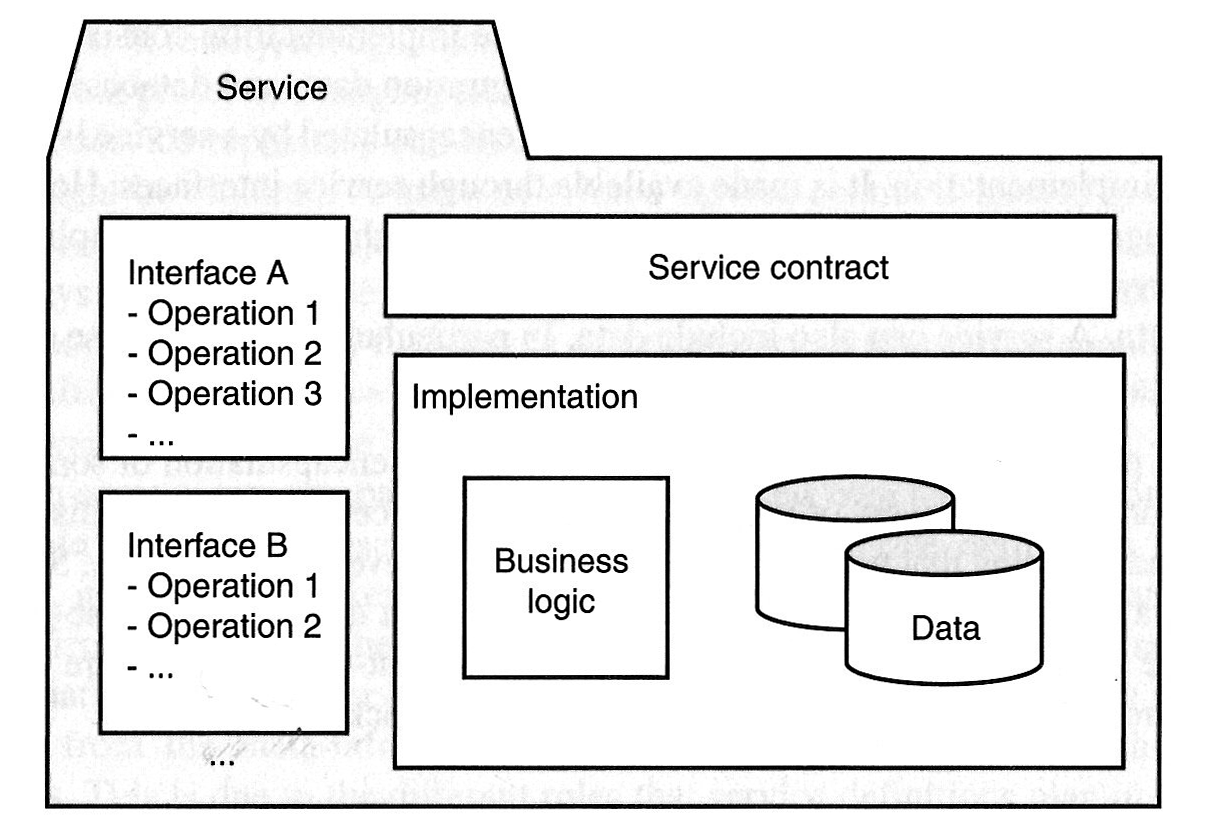
\includegraphics[scale=1.0]{service_structure.png}
\caption{Structure of a service with the relations of the particular artefacts \cite[p.45]{krafzig}.}
\label{fig:service}
\end{figure}




\subsection{Services at different layers of implementation}
\label{ch:service_layers}
The system layers specified in \ref{ch:system_layers} serve as basis for the assignment of services to different levels of implementation.

\subsubsection{Chip Layer}
The chip layer is the lowest layer of implementation and contains very generic services which are used by higher layers in order to create more advanced services. In various sources this layer is referred to as the core-, or platform layer. In accordance with that the services at this layer are denoted core services \cite[p.44]{genesys}.

Typical examples for services located at this level are message based 
communication services for the interaction of system elements, global time base services or mechanisms to compose the overall system out of the independently developed components. Such mechanisms include fault isolation services and clock synchronization services \cite[p.7-12]{genesys}. In other words, the chip layer provides a platform where recurring problems can be dealt with once and for all.

\subsubsection{Device Layer}
The device layer contains more advanced hardware parts. With respect to figure \ref{fig:service_levels} these might be sensors, actuators, ADCs (Analog-to-digital converters), AURIX chips, the CAN bus (Controller area network) or a WDT (Watchdog Timer). Since there is no consistent denomination for the services located at this layer, they are referred to as \emph{device services} within this thesis.

Device services make use of the underlying core services and other services at the device layer in order to provide their intended functionality. 
An acceleration sensor, for example, could make use of an ADC, which in turn operates with a platform service for the time, for generating periodic sampling points.

\subsubsection{System Layer}
The highest layer is the system layer, containing the most advanced services, which are usually provided to the end user. Same as with the device services, there is no uniform denomination for services at this layer throughout literature. Thus, they are denoted \emph{system services}.

System services emerge by binding together services of lower layers. An example for a system service could be a passive safety service for breaking or searing, which bases on an acceleration measurement service and other device services.
\\
\\
Figure \ref{fig:service_levels} features an example of which hardware parts may belong to which integration layer with respect to the considered system vehicle. 


\begin{figure}[!htbp]
\centering
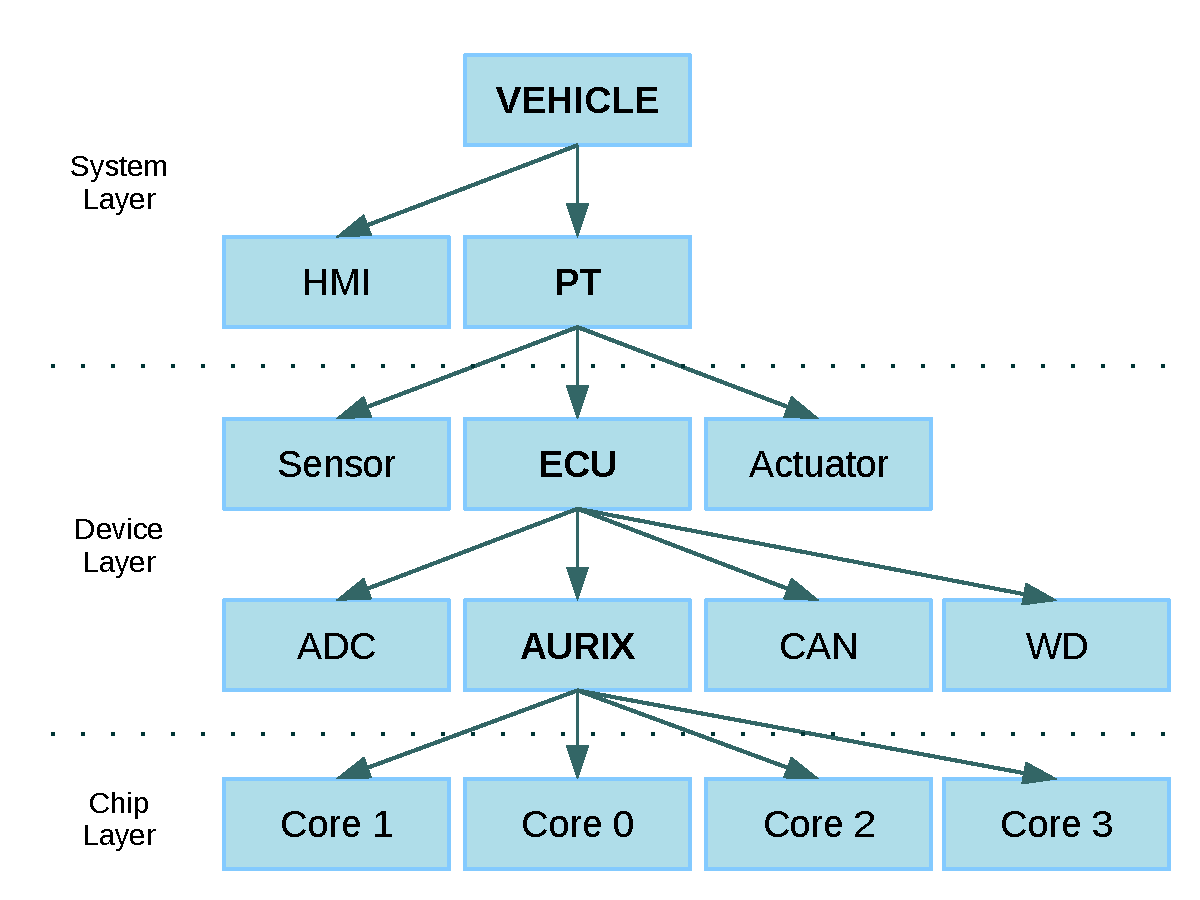
\includegraphics[scale=0.6]{service-levels.pdf}
\caption{Examples of hardware parts at different levels \cite{avl}}
\label{fig:service_levels}
\end{figure}









\section{Architecture}

\label{ch:architecture}

The term architecture is very generic and has various different domains, like \emph{hardware architecture}, \emph{software architecture}, \emph{system architecture} or \emph{enterprise architecture}. In general architecture is concerned with how the components of a system can be arranged and interrelated in order to assemble an overall system \cite{ISO_42010} \cite{ning}. 

Within the \mbox{ISO/IEC/IEEE 42010} standard the term architecture is referred to by ``fundamental concepts or properties of a system in its environment embodied in its elements, relationships, and in the principles of its design and evolution'' \cite{ISO_42010}. The \emph{fundamental concepts} are thereby system element (cf. section \ref{sec:system_element}), the relations inside the system, the relations to the environment and the principles of design and evolution.

This definition applies for any kind of architecture, but the emphases on these concepts vary with respect to the considered domain. The software architecture usually focuses very much on the system elements, while the enterprise architecture is more concerned with the principles \cite{ISO_42010}.

This is in compliance with the definition by AUTOSAR:
\begin{quote}
``The fundamental organization of a system embodied in its components, their static and dynamic relationships to each other, and to the environment, and the principles guiding its design and evolution'' \cite{autosar_glossary}.
\end{quote}

In \cite{rodrigues2011} it is stated that the ``relationship and principles of design of the components, functions and the interface established between subsystems can also be defined by architecture'' \cite{rodrigues2011}.

The definition presented below is compatible with all kinds of architecture design, for they share the same basic principles.

\begin{myquote}
An architecture is a systematic description of the structure of a system by means of its involved components and their relations to each other, and specifies also the connections and interactions of a system to its environment.

At the same time, architecture is also responsible for determining the principles of design and evolution.
\end{myquote}


\subsection{Demarcation from related terms}
The placement of architecture in relation to other entities like system or environment (cf. chapter \ref{ch:system}) is illustrated in figure \ref{fig:architecture_ontology}. 

\begin{description}
\item [Architecture description.]
	Many sources mix up the definitions of architecture and architecture description, what is a recurring source of confusion. In contrast to the actual architecture of a system, the term architecture description denotes the artefacts which document the respective architecture \cite{ISO_42010}. Their relation is also pictured in figure \ref{fig:architecture_ontology}.

	According to the \mbox{ISO/IEC/IEEE 42010} standard, the architecture description is used to express the architecture of a system of interest by means of the following elements:
	\begin{itemize}
	\item Specification of the purposes of the system,
	\item Suitability for achieving these purposes,
	\item Feasibility of construction and applicability,
	\item Maintainability,
	\item Evolvability and
	\item Association of these concerns with the stakeholders having these concerns \cite{ISO_42010}.
	\end{itemize}
	One and the same architecture can be described by several different architecture descriptions, and at the same time an architecture description can also characterise multiple architectures \cite{ISO_42010}.

\item [Stakeholder.]
	The stakeholders are all people, which are somehow related to the system and have any interest in the system. Those include users, operators, owners, developers, maintainers and others \cite{ISO_42010}.

\item [System concern.]
	A specific system concern can be held by one more more stakeholders and can appear in various different forms, e.g. expectations, responsibilities, requirements, assumptions, dependencies and more \cite{ISO_42010}. 

\item [Purpose.]
	Purposes are one kind of system concerns, which are issued by the stakeholders \cite{ISO_42010}.
\end{description}

\begin{figure}[!htbp]
\centering
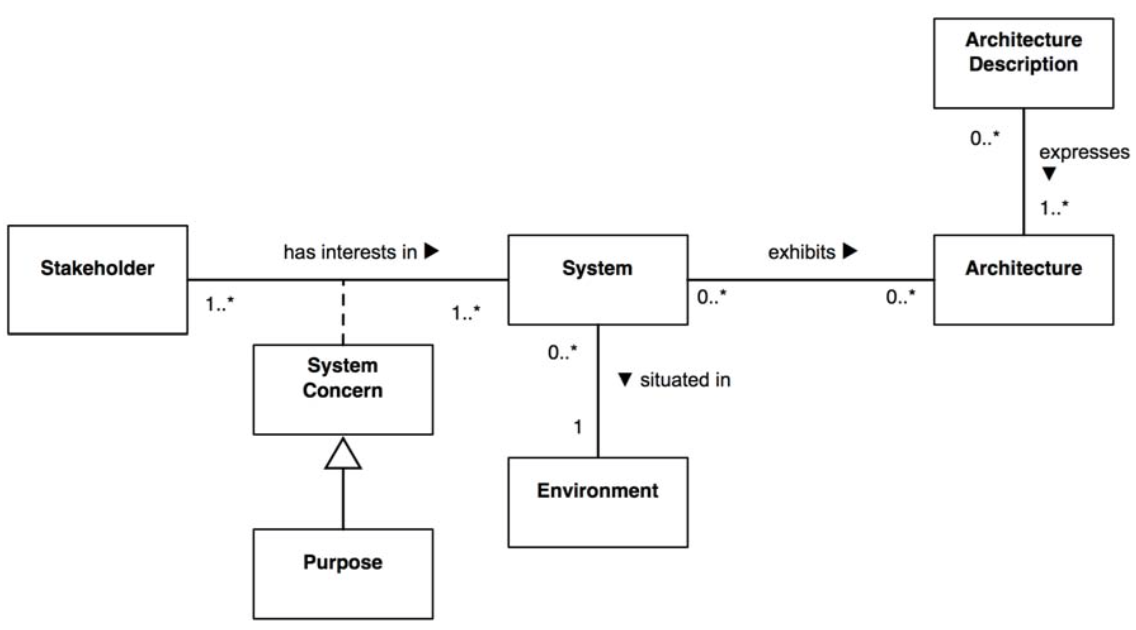
\includegraphics[scale=0.35]{architecture_ontology.png}
\caption{Relations of architecture to other entities \cite{ISO_42010}}
\label{fig:architecture_ontology}
\end{figure}










\section{Service oriented architecture}
\label{ch:soa}

The term service oriented architecture has been widely used for marketing and praising new products. This resulted in various misinterpretations of the term, because some vendors suggested that a SoA is something that can be bought or installed on an existing system, missing the point that SoA is not a product, but a set of design paradigms that can be applied on architectures.

The driving factor for the application of this design paradigm are certain benefits that come with the modularization of software. Those are not only reduction of development costs, but, with respect to embedded systems also a saving in hardware components \cite{sommer}. Furthermore, it increases flexibility, scalability and fault tolerance, enabling a system to run, even if parts are erroneous or down \cite[p.33]{rosen} \cite[p.17-18]{josuttis}.
\\
\\
Different authors and companies explain the term from different viewpoints and with different focuses.

\begin{description}
	\item [OASIS.]
	OASIS is a non-profit consortium that drives the development, convergence and adoption of open standards for the global information society.
	\begin{quote}
	\emph{``A paradigm for organizing distributed capabilities that may be under the control of different ownership domains. It provides a uniform means to offer, discover, interact with and use capabilities to produce desired effects consistent with measurable preconditions and expectations''} \cite{oasis2006}.
	\end{quote}

	\item [Papazoglou.]
	\begin{quote}
	\emph{``Service-oriented architectures (SOA) is an emerging approach that addresses the requirements of loosely coupled, standards-based, and protocol independent distributed computing''} \cite{papazoglou2007}.
	\end{quote}

	\item [Donini, Marrone et al.]
	\begin{quote}
	\emph{``SOA is an architectural style for building software applications that use services available in a network such as the web and it represents the widest accepted model to design geographical distributed systems.''} - \cite{donini2008}
	\end{quote}

	\item [Arcitura.]
	\begin{quote}
	\emph{``Service-oriented architecture is a technology architectural model for service-oriented solutions with distinct characteristics in support of realizing service-orientation and the strategic goals associated with service-oriented computing''} \cite{arcitura}.
	\end{quote}
\end{description}

The definition below emerged as result of extensive investigations in this research area. In contrast to all the other definitions, which are somehow biased due to their relation to a certain area of industry, this one is quite generic and may be used for any kind of SoA. In case of embedded- or safety-critical systems, there are of course additional characteristics which are crucial.

\begin{myquote}
	The service oriented architecture is no actual design, which can be simply implemented or installed, but a collection of design principles for distributed systems.

	Originating from the object oriented- and component based engineering, it pushes the concept of software reuse to a new level by using technology independent and loosely coupled services.

	Accordingly, a SoA disposes of an arbitrary number of services, which are interconnected by means of an underlying network and predefined protocols.
\end{myquote}

As stated, SoA is no specific implementation but a set of rules to achieve a certain target state. The final implementation can therefore consist of multiple technologies, products, Application Programmers Interfaces (APIs) and supporting infrastructures \cite[p.29]{erl2011}. This enables an unproblematical exchange of components by components of other vendors, as long as the provided services remain unaffected.

A SoA is not just a simple collection of services, but offers also composition mechanisms for services. Those enable the creation of agile, higher-level services with a more sophisticated functionality, without having to build everything from scratch. \cite[p.12]{josuttis}.



\subsection{Historic Development}
The term \emph{service oriented architecture} first appeared in 1996 \cite[p.7]{rosen}. It emerged from the CBSE (cf. figure \ref{fig:software_reuse}) and was more or less an improvement, for it allowed the components to be wider distributed and looser coupled. However, since both approaches feature certain advantages, both of them have been developed in parallel ever since, resulting in many similarities, but also many differences \cite{breivold}. 


\begin{figure}[!htbp]
\centering
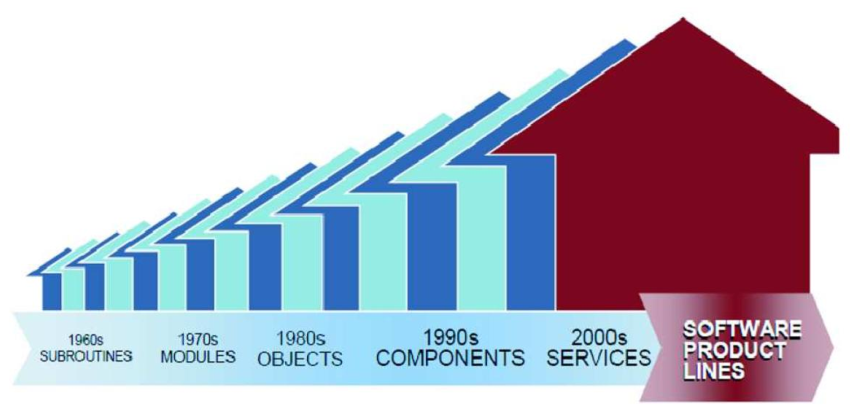
\includegraphics[width=\textwidth]{software_reuse.pdf}
\caption{Development of software reuse concepts from the 1960 to present \cite{clements}.}
\label{fig:software_reuse}
\end{figure}


\subsection{Structure of a SoA}
\label{sec:structure_of_soa}
The four main artefacts of a SoA are service provider, service consumer, service repository and the service contract \cite{arrowhead} \cite{breivold} \cite{rodrigues2011}. There are also alternative terms for those, which are mentioned here, but throughout this thesis the previously stated terms will be used.

\begin{description}
\item [Service provider/ Service Owner.] 
The task of the service provider is to provide a service and its functionality. Additionally, he should formulate the service description in form of a contract, which is then handed over to the service repository in order to make the service discoverable \cite{breivold}.

\item [Service Repository/ Service Registry/ Service Directory.]
The service repository is, more or less, a database of services, which may be distributed. It disposes of certain publishing mechanisms in order to make services discoverable by the . Therefore it contains all the information from the (of every version of the service), as well as meta information like physical location, provider information, technical constraints, security issues and of course the link to the registered service. \cite[p.60-61]{krafzig} \cite{breivold} \cite{converge}.

Services can be added to, or taken from, the service repository dynamically. Thus, services need to be already running and ready to use in order to be discovered and composed at runtime.

\item [Service Consumer/ Service Client/ Service Requester.]
The service consumer is the instance that calls the service and can be either an end-user or another service. He sends a request for searching the service repository for specific services by the service interface description. Subsequently, the repository returns a list with suitable services. If an appropriate service is identified the service consumer creates a dynamic binding with the service provider in order to invoke the service and interact with it \cite{breivold} \cite{converge}. This procedure is depicted in figure \ref{fig:service_cronology}.

\item [Service Contract.]
The service contract is described in detail in section \ref{sec:service_structure}. It is handed over to the service repository from the service provider.

\item [Service Inventory.]
Erl, Bennett et al. mention this additional term in connection with SoA. According to their definition, ``A service inventory is an independently standardized and governed collection of complementary services within a boundary that represents an enterprise or a meaningful segment of an enterprise'' \cite[p.41]{erl2011}. 

The term enterprise in this definition appears a bit bizarre and is a result of the research area related with this source. For the scope of this thesis the boundary is defined as the vehicle. Thus, the service inventory includes all services which could be provided by the vehicle. The difference to the service repository is that the service does not need to be available, or even implemented. Instead, it is a static list of developed or conceived services.
\end{description}

The relations of the various artefacts are depicted in figure \ref{fig:soa_overview}.

\begin{figure}[!htbp]
\centering
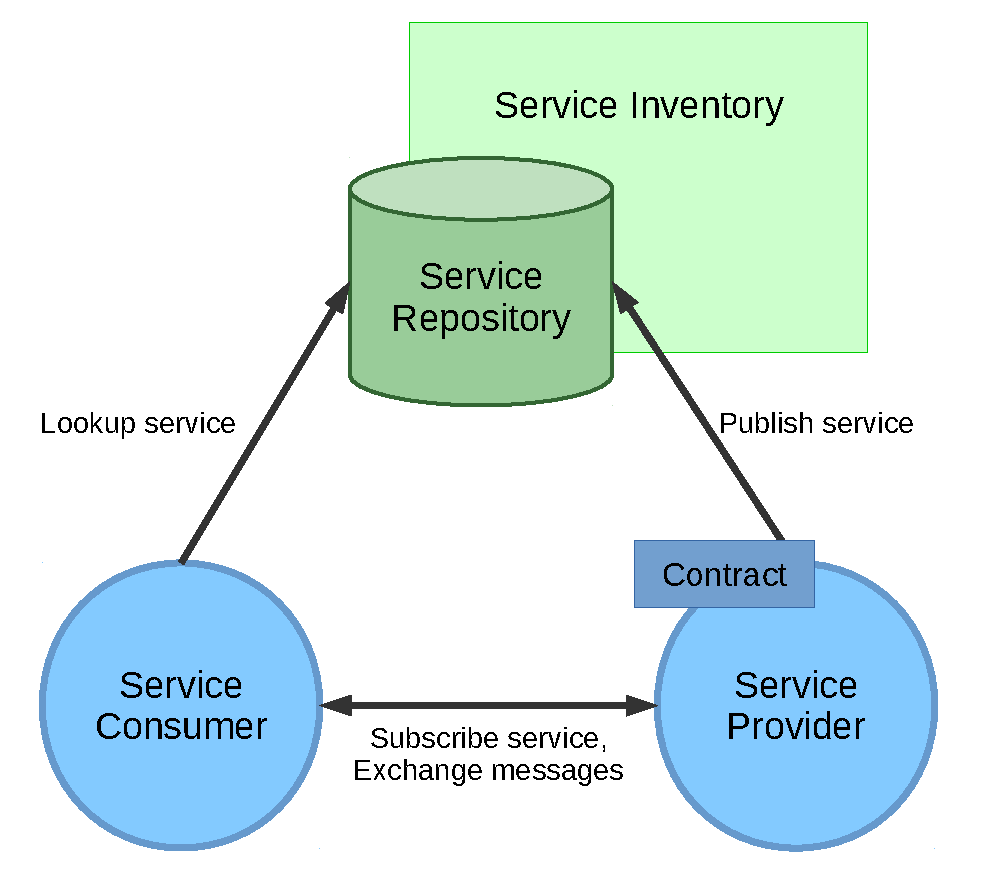
\includegraphics[scale=0.6]{soa-architecture.pdf}
\caption{Relation of \emph{service provider}, \emph{service consumer} and \emph{service repository} \cite{arrowhead} \cite{converge}}
\label{fig:soa_overview}
\end{figure}

\begin{figure}[!htbp]
\centering
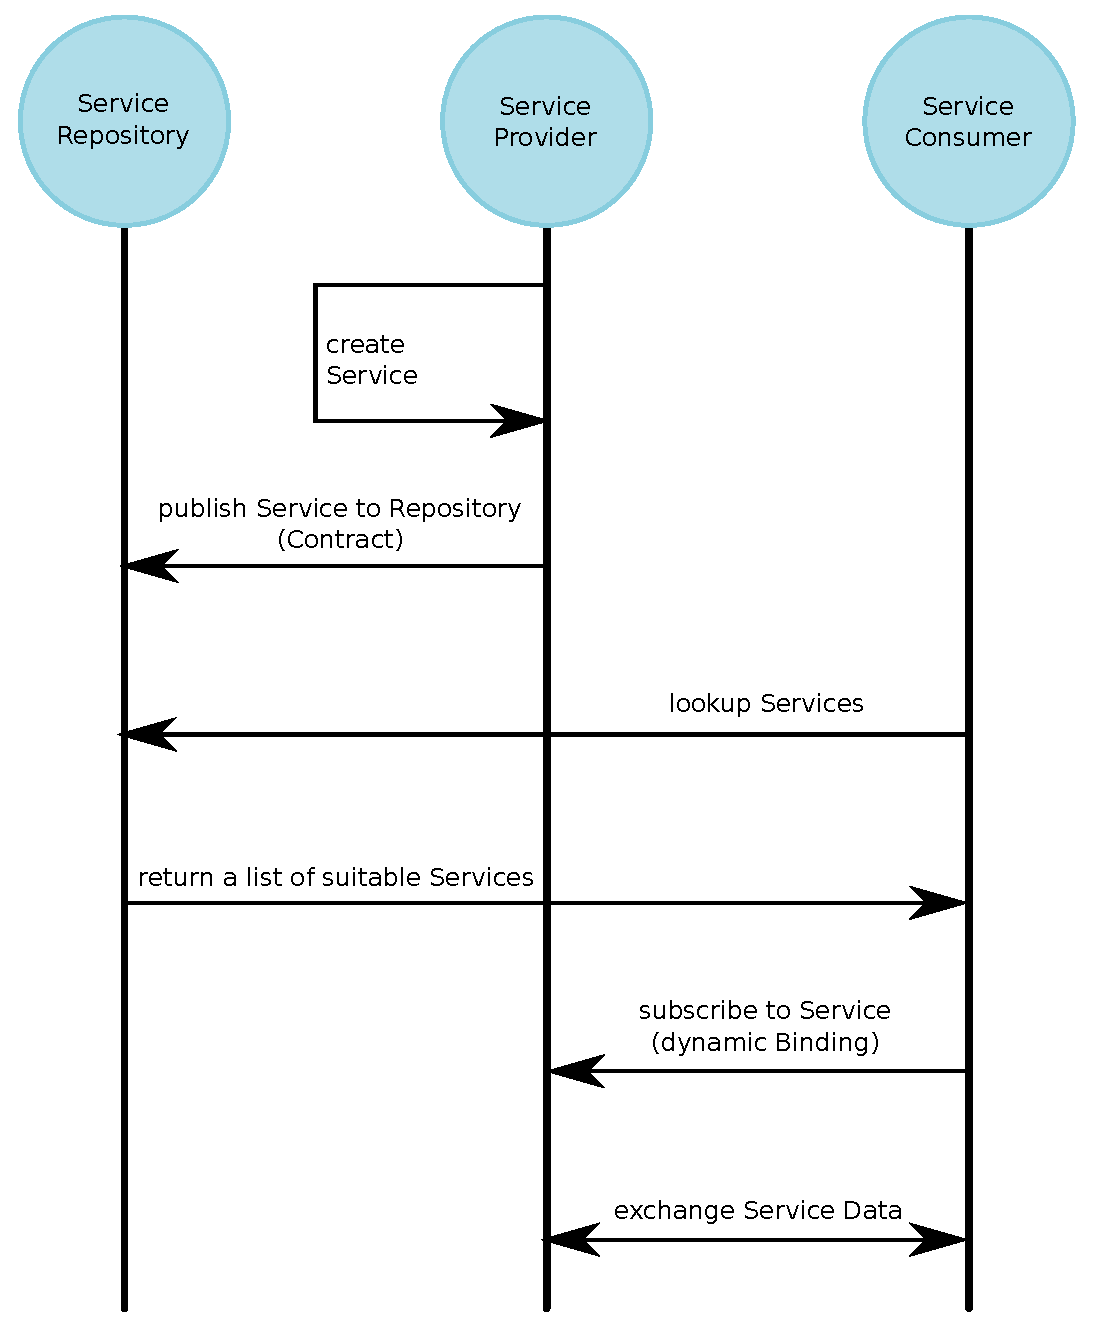
\includegraphics[scale=0.8]{soa_process.pdf}
\caption{Chronology of how a service is used in a SoA \cite{converge}.}
\label{fig:service_cronology}
\end{figure}











\section{Dependability}

The terms availability and reliability, which can be found at any level of implementation, are closely tied and usually come together. Often, they are also coupled with the term maintenance, which also plays an important role in the design of any system \cite[p.116]{genesys} \cite{lessner}.

\subsection{Reliability}
\label{sec:reliability}

Reliability denotes the time an element needs to fail while its operating. In other words it is ``the probability of the failure-free operation of a system for a specific period of time in a specific environment'' \cite[p.116]{genesys}. Nelson describes it more technically as ``Reliability, $R(t)$, is the conditional probability that a system can perform its designed function at time $t$, given that it was operable at time $t=0$'' \cite{nelson}.

In terms of services, the reliability can be enhanced by the ability to recover state information after an interruption and continue the service as it has never been interrupted \cite{genesys}. The reliability of higher level elements is of course limited by the reliability of its sub elements.


\subsection{Availability}

\label{sec:availability}
The definition of availability is ambiguous. The \mbox{ISO 26262} standard defines the availability as the ``capability of a product to be in a state to execute the function required under given conditions, at a certain time or a given period, supposing the required external resources are available'' \cite{iso26262:1}. Obermaisser and Kopetz, however, describe it as the ``probability of a software service or system being available when needed'' \cite[p.116]{genesys}, which is very similar to the definition found in \cite{lessner} and \cite{nelson}.

The difference here is that the prior denotes availability as the availability of an element at this very moment, while the latter defines it as a probability of an element to be operational and ready to use.

Two important terms which come in connection with availability are MTTF (Mean Time To Failure), the expected time until the system fails, and MTTR (Mean Time To Repair), the necessary time to restore a failed system to normal operation. The availability $A$ can then be expressed as $A = MTTF/(MTTF + MTTR)$ \cite{nelson}. 

The availability characteristics of a system are represented by its reliability and maintainability. Accordingly, even highly reliable entities can have a poor availability if the repair time of its sub entities takes very long \cite{lessner}. The availability can be improved by the application of dedicated \emph{fault tolerance mechanisms} (cf. section \ref{ch:fault_tolerance}) \cite{nelson}.















\section{Functional safety}
\label{ch:functional_safety}

The term safety denotes the absence of an unreasonable risk \cite{iso26262:1}. Systems which operate with people and could endanger those in case of a malfunction have certain safety requirements in addition to functional requirements. Those safety requirements are issued by dedicated standards like the \mbox{ISO 26262} standard. In accordance with that the \mbox{ISO 26262} standard describes functional safety as the ``absence of unreasonable risk due to hazards caused by malfunctioning behaviour of E/E systems'' \cite{iso26262:1}. Risk, in turn, is defined as the product of the \emph{probability of occurrence} and the \emph{severity of harm} \cite{iso26262:1}.

In contrast to security, functional safety only addresses the absence of risk due to equipment malfunction. It does not care about possible risks due to malicious events caused by other people, or just inappropriate operation of the user.


\subsection{Disambiguation safety and security}
Two terms which often appear together and appear very much alike are \emph{safety} and \emph{security}. Nevertheless, they have a completely different meaning in technical systems.

The term \emph{safety} denotes the ``absence of an unreasonable risk'' \cite{autosar_glossary} \cite{iso26262:1} and is concerned with correct operation of the equipment in a specific system. Therefore, it is concerned with things like \emph{error detection}, \emph{fault prevention}, \emph{failure migration}, \emph{diagnosis} and similar.

\emph{Security}\index{security} is concerned with preventing unauthorized access, or unexpected input. AUTOSAR defines the term as \emph{``Protection of data, software entities or resources from accidental or malicious acts''} \cite{autosar_glossary}. With the advance of software and interconnection in vehicles, \emph{security} becomes more and more of an issue, because all the functionality in a car, even highly critical like an automatic brake system or a collision warning system will be approachable through a network. Especially, if the vehicle gets connected to any proprietary network like the Internet. With the advance of the service oriented architecture paradigm for automotive, it is planed to run remote diagnosis and firmware updates over the air. This is an obvious weak point and an exploit of this can affect the operation of the vehicle and the safety of the driver \cite{nilsson2008}.

Although, \emph{safety} and \emph{security} are separate disciplines, for automotive the functionalities cannot be classified into safety or security relevant functionality, but has always aspects of both disciplines at the same time \cite{nilsson2008}. Nevertheless, this thesis is mostly representing the \emph{safety} oriented point of view.


\subsection{Safety related terminology}
\label{sec:fault,error,failure}
\emph{Fault}, \emph{error} and \emph{failure} are terms with are often mixed up and used in the same context, since they seem to be very similar in their meaning. Nevertheless, they stand for different things and their disambiguation is crucial.


\begin{description}
\item [Fault.]
In \mbox{ISO 26262} standard a \emph{fault} is listed as an ``abnormal condition that can cause an element or an item to fail'' \cite{iso26262:1} \cite{autosar_glossary}. 

Faults come in different forms. An \emph{intermittent fault} occurs from time to time and disappears without any repair measures taken place. This is typical for hardware components which are worn out and almost breaking down. \emph{Transient faults}, on the other hand, appear once, and do not recur afterwards. This is for example the case if there is some electromagnetic interference. \emph{Permanent faults} naturally remain until the faulty component is exchanged or repaired \cite{iso26262:1}.

A term related to fault, is \emph{fault coverage}. It denotes ``the number of the faults detected as a percentage of the total number of faults affecting the system'' \cite{elattar2007}.


\item [Error.]
An error is the deviation of a computed, observed or measured value or condition and the expected, theoretically correct value. An error occurs as consequence of unexpected operating conditions or a fault.
Nevertheless, a fault does not necessarily lead to an error \cite{iso26262:1} \cite{nelson} \cite{autosar_glossary}. If the error exceeds a certain threshold it can cause a failure \cite{autosar_glossary}.

There are two different classifications of errors. They can be divided into \emph{soft-} and \emph{hard errors} or \emph{data-} and \emph{control flow errors} \cite{israr2014} \cite{elattar2007}.
	\begin{description}
	\item [Soft Error.]
	Soft errors occur when a temporary extra charge is induced into the electric circuit. Usually it is due to cosmic radiation and causes a flip of the data state in a memory element \cite{israr2014} \cite{elattar2007}.

	This kind of error will become even more severe in the future, due to the decreasing size of electronic logic, as well as their increasing complexity \cite{elattar2007}.

	\item [Hard Error.]
	In contrast to soft errors, hard errors are caused by a constant property change of an electric component. This could happen either because of a change in the input temperature, or input voltage \cite{israr2014}.
	\end{description}

	\begin{description}
	\item [Data Error.]
	This error means a change of the data stored any memory location or register \cite{elattar2007}.

	\item [Control Flow Error.]
	A control flow error leads to wrong execution sequence of instructions. This is the case, when the memory storing the address of the next execution instruction is changed \cite{elattar2007}.
	\end{description}

\item [Failure.]
\emph{Failure} denotes that an element is not able to provide its functionality any longer. This happens usually due to errors in the element or the environment, which are in turn caused by various faults \cite{iso26262:1} \cite{nelson} \cite{autosar_glossary}.

The averaged frequency of occurrence of a failure is denoted \emph{failure rate}. It is counted in \emph{hours of operation until a serious fault} - e.g. 10e5 to 10e9 hours of operation \cite{rodrigues2011}.

Another term which frequently comes up in connection with failure, is \emph{failure mode}. This denotes, depending on the consulted source, either the manner in which the component fails \cite{international2006analysis}, or the manner by which a occurred fault is observed \cite{mil1980}.
\end{description}




\section{Fault tolerance}
\label{ch:fault_tolerance}

The key concept of a \emph{fault tolerant} design is to enable a system to provide its intended functionality in the presence of a given number of faults \cite{nelson}.

Thus, the fault tolerance mechanisms are not responsible for preventing the occurrence of faults, but assure that a fault does not lead directly to the violation of the safety goals, which maintain the system in a safe state \cite{iso26262:1}. Possible fault include not only internal faults like design-faults or hardware wear-outs, but also external ones. For example misuse by the user or cosmic radiation. Fault tolerance mechanisms have become indispensable for advanced electric systems, because due to the billions of transistors present and the various circumstances circumstances, which can lead to faults, faultless systems remain an utopian dream \cite{genesys}.



\subsection{Design of fault tolerant Systems}
The prerequisite for designing a fault tolerant system is a so called \emph{fault hypothesis}, which is an assumption regarding the type and frequency of faults the system is supposed to handle.

These can include
\begin{itemize}
\item \emph{Software error} - Especially for complex software it can be assumed that there are a certain amount of bugs and imprecisions.
\item \emph{Delay and disruption error} - This is relevant for all networking systems.
\item \emph{Transient faults} - This means a possible corruption of Flip-Flops or memory cells with the progression of time.
\end{itemize}
